% !TeX root = ../main.tex
% Add the above to each chapter to make compiling the PDF easier in some editors.

\chapter{Analysis}

In this chapter, we study functions $f: \sS \to \R$ where $\sS \subseteq \R^n$.

\section{First-order Taylor Approximations}

\begin{defn}[Gradient] The \emph{gradient}\index{gradient} of a function $f: \sS \to \R$ at point $\vx \in \sS$ is, \begin{align}
    \grad f(\vx) \defeq \trans{\begin{bmatrix}
        \pdv{f(\vx)}{\vx(1)} & \cdots & \pdv{f(\vx)}{\vx(n)}
    \end{bmatrix}}.
\end{align}
\end{defn}

For a single-variable function $f: \R \to \R$ that is differentiable, we have for any $x, \delta \in \R$, \begin{align*}
    f(x + \delta) = f(x) + \odv{f(x)}{x} + o(|\delta|), \quad \text{where } \lim_{\delta \to 0} \frac{o(|\delta|)}{|\delta|} = 0,
\end{align*} using a first-order Taylor approximation around $x$. We can use a similar approximation when $f$ is a multi-variable function.

\begin{defn}[Fréchet differentiable] A function $f: \sS \to \R$ is \emph{(Fréchet) differentiable}\index{Fréchet differentiable} at $\vx \in \sS$ if there exists $\vg \in \R^n$ such that,\footnote{Here, $\vg$ can be understood as a candidate for $\grad f(\vx)$ and $f(\vx) + \trans{\vg}\vdelta$ is a linear approximation of $f$ around $\vx$.} \begin{align}
    \lim_{\substack{\vdelta \in \R^n \\ \vdelta \to \vZero}} \frac{|f(\vx + \vdelta) - [f(\vx) + \trans{\vg}\vdelta]|}{\norm{\vdelta}_2} = 0.
\end{align} This is equivalent to, \begin{align}
    f(\vx + \vdelta) = f(\vx) + \trans{\vg}\vdelta + o(\norm{\vdelta}_2),
\end{align} for any $\vx \in \sS$ and $\vdelta \in \R^n$ where $\lim_{\vdelta \to \vZero} \frac{o(\norm{\vdelta}_2)}{\norm{\vdelta}_2} = 0$. This is also called a \emph{first-order expansion}\index{first-order expansion} of $f$ around $\vx$.
\end{defn}
\begin{rmk}
If this holds, $\vg = \grad f(\vx)$.
\end{rmk}

\begin{defn}[Continuously differentiable] We say that $f : \sS \to \R$ is \emph{continuously differentiable}\index{continuously differentiable} on $\sS$ if it is differentiable and its gradient is continuous on $\sS$.
\end{defn}

\begin{thm}[Taylor's theorem, multivariate first-order remainder form]\index{Taylor's theorem (first-order)} If $f: \sS \to \R$ is continuously differentiable, then for all $\vx, \vy \in \sS$, \begin{align}
    f(\vy) = f(\vx) + \trans{\grad f(\vz)}(\vy - \vx),
\end{align} for some $\vz \in [\vx, \vy] \defeq \{\theta\vx + (1-\theta)\vy \mid \theta \in [0,1]\}$.
\end{thm}\begin{marginfigure}
\centering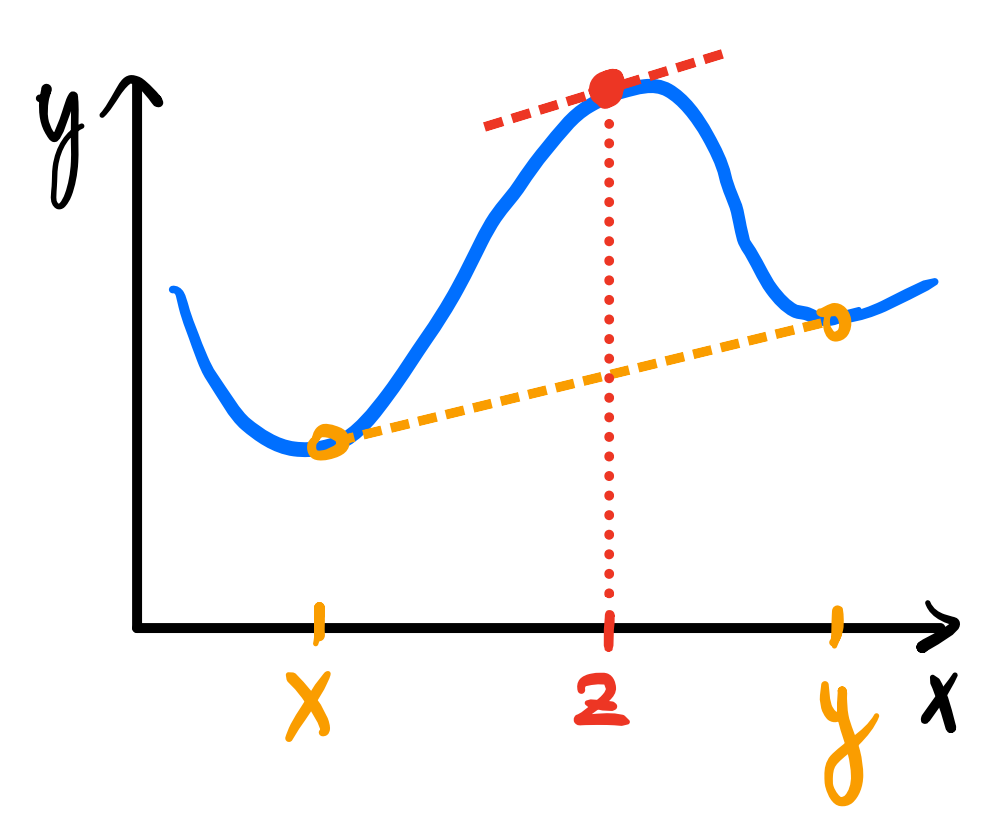
\includegraphics[width=3cm]{notes/figures/taylors_theorem.png}
\caption{Illustration of Taylor's theorem. The affine approximation is shown in orange.}
\end{marginfigure}\noindent Taylor's theorem implies that $f$ can be approximated by the affine function, \begin{align*}
    \vy \to f(\vx) + \trans{\grad f(\vx)}(\vy - \vx),
\end{align*} when $\vy$ is ``close to'' $\vx$.

\section{Directional Derivatives}

\begin{defn}[Directional derivative] Let $f: \sS \to \R$ be differentiable at $\vx \in \R^n$. Given $\vd \in \R^n$, the \emph{directional derivative}\index{directional derivative} of $f$ at $\vx$ in the direction $\vd$ is, \begin{align}
    D f(\vx)[\vd] \defeq \lim_{\lambda \to 0} \frac{f(\vx + \lambda\vd) - f(\vx)}{\lambda}.
\end{align}
\end{defn}

\begin{lem} $D f(\vx)[\vd] = \trans{\grad f(\vx)}\vd$.
\end{lem}
\begin{proof} Using a first-order expansion, we have, \begin{align*}
    f(\vx + \lambda\vd) = f(\vx) + \lambda \trans{\grad f(\vx)}\vd + o(\lambda \norm{\vd}_2).
\end{align*} Dividing by $\lambda$ yields, \begin{align*}
    \frac{f(\vx + \lambda\vd) - f(\vx)}{\lambda} = \trans{\grad f(\vx)}\vd + \underbrace{\frac{o(\lambda\norm{\vd}_2)}{\lambda}}_{\to 0}.
\end{align*} Taking the limit $\lambda \to 0$ gives the desired result.
\end{proof}

\subsection{First-order Optimality Conditions}

\begin{defn}[Stationary point] Given a function $f: \sS \to \R$, a point $\vx \in \sS$ where $\grad f(\vx) = 0$ is called a \emph{stationary point}\index{stationary point} of $f$.\footnote{Being a stationary point is not sufficient for optimality. Take for example the point $x \defeq 0$ of $f(x) \defeq x^3$.}
\end{defn}

\begin{thm}[First-order optimality condition]
If $\vx \in \sS$ is a local extremum of a differentiable function $f: \sS \to \R$, then $\grad f(\vx) = 0$.\footnote{Here it is important that we have chosen $\sS \subseteq \R^n$ to be open. When $\sS$ is not open, an extremum could be on the boundary of the domain, where the gradient is non-zero.}
\end{thm}
\begin{proof}
    Assume $\vx$ is a local minimum of $f$. Then, for all $\vd \in \R^n$ and for all small enough $\lambda \in R$, we have $f(\vx) \leq f(\vx + \lambda\vd)$, so, \begin{align*}
        0 &\leq f(\vx + \lambda\vd) - f(\vx) \\
        &= \lambda \trans{\grad f(\vx)}\vd + o(\lambda\norm{\vd}_2). \margintag{using a first-order expansion of $f$ around $x$}
    \end{align*} Dividing by $\lambda$ and taking the limit $\lambda \to 0$, we obtain, \begin{align*}
        0 \leq \trans{\grad f(\vx)}\vd + \lim_{\lambda \to 0}\frac{o(\lambda\norm{\vd}_2)}{\lambda} = \trans{\grad f(\vx)}\vd.
    \end{align*} Take $\vd \defeq - \grad f(\vx)$.\footnote{We can only take this step because we assumed that $\sS$ is open.} Then, $0 \leq - \norm{\grad f(\vx)}_2^2$, so $\grad f(\vx) = 0$.
\end{proof}

\section{Second-order Taylor Approximations}

\begin{defn}[Jacobian] Given a vector-valued function, \begin{align*}
    \vg: \R^n \to \R^m, \quad \vx \mapsto \begin{bmatrix}
        g_1(\vx) \\
        \vdots \\
        g_m(\vx) \\
    \end{bmatrix},
\end{align*} where $g_i: \R^n \to \R$, the \emph{Jacobian}\index{Jacobian} of $\vg$ at $\vx \in \R^n$ is, \begin{align}
    D \vg(\vx) \defeq \begin{bmatrix}
        D g_1(\vx) \\
        \vdots \\
        D g_m(\vx) \\
    \end{bmatrix} \defeq \begin{bmatrix}
        \pdv{\vg(\vx)}{\vx(1)} & \cdots & \pdv{\vg(\vx)}{\vx(n)}
    \end{bmatrix}.
\end{align}
\end{defn}
\begin{rmk} For $f: \sS \to \R$ and any $\vx \in \sS$, $D f(\vx) = \trans{\grad f(\vx)}$.
\end{rmk}
\begin{ex}
Given $f: \sS \to \R$ and any $\vx \in \sS$, consider the vector-valued function $\grad f$. We have, \begin{align}
    D \grad f(\vx) = \begin{bmatrix}
        \pdv{\grad f(\vx)}{\vx(1)} & \cdots & \pdv{\grad f(\vx)}{\vx(n)}
    \end{bmatrix} = \begin{bmatrix}
        \pdv{f(\vx)}{\vx(1),\vx(1)} & \cdots & \pdv{f(\vx)}{\vx(n),\vx(1)} \\
        \vdots & \ddots & \vdots \\
        \pdv{f(\vx)}{\vx(1),\vx(n)} & \cdots & \pdv{f(\vx)}{\vx(n),\vx(n)}
    \end{bmatrix}. \label{eq:jacobian_hessian}
\end{align}
\end{ex}

\begin{defn}[Hessian] Given $f: \sS \to \R$ that is twice differentiable coordinatewise, we define the \emph{Hessian}\index{Hessian} $\mH_f(\vx) \in \R^{n \times n}$ of $f$ at a point $\vx \in \sS$ as, \begin{align}
    \mH_f(\vx)(i,j) \defeq \pdv{f(\vx)}{\vx(i),\vx(j)}
\end{align}
\end{defn}
\begin{rmk} By \cref{eq:jacobian_hessian}, $\mH_f(\vx) = \trans{(D \grad f(\vx))}$.\footnote{Sometimes, $\mH_f(\vx) = \grad^2 f(\vx)$ is written (informally!).}
\end{rmk}

\begin{defn}[Twice Fréchet Differentiable] We say a function $f: \sS \to \R$ is \emph{twice (Fréchet) differentiable}\index{twice Fréchet differentiable} at $\vx \in \sS$ if there exists $\vg \in \R^n$ and a matrix $\mM \in \R^{n \times n}$ such that,\footnote{You can think of $\vg$ as a candidate for $\grad f(\vx)$, $\mM$ as a candidate for $\mH_f(\vx)$, and $f(\vx) + \trans{\vg}\vdelta + \frac{1}{2}\trans{\vdelta}\mM\vdelta$ is a quadratic approximation of $f$ around $\vx$.} \begin{align}
    \lim_{\substack{\vdelta \in \R^n \\ \vdelta \to \vZero}} \frac{|f(\vx + \vdelta) - [f(\vx) + \trans{\vg}\vdelta + \frac{1}{2}\trans{\vdelta}\mM\vdelta]|}{\norm{\vdelta}_2^2} = 0.
\end{align} This is equivalent to, \begin{align}
    f(\vx + \vdelta) = f(\vx) + \trans{\vg}\vdelta + \frac{1}{2}\trans{\vdelta}\mM\vdelta + o(\norm{\vdelta}_2^2),
\end{align} for any $\vx \in \sS$ and $\vdelta \in \R^n$ where $\lim_{\vdelta \to \vZero} \frac{o(\norm{\vdelta}_2^2)}{\norm{\vdelta}_2^2} = 0.$ This is also called a \emph{second-order expansion}\index{second-order expansion} of $f$ around $\vx$.
\end{defn}
\begin{rmk}
If this holds, \begin{enumerate}
    \item $\vg = \grad f(\vx)$,
    \item $\mM = \mH_f(\vx)$, and
    \item $\mH_f(\vx) = \trans{\mH_f(\vx)}$.
\end{enumerate}
\end{rmk}

\begin{defn}[Twice continuously differentiable] We say that $f: \sS \to \R$ is \emph{twice continuously differentiable}\index{twice continuously differentiable} on $\sS$ if it is twice differentiable and the gradient and Hessian are continuous on $\sS$.
\end{defn}

\begin{thm}[Taylor's theorem, multivariate second-order remainder form]\index{Taylor's theorem (second-order)} If $f: \sS \to \R$ is twice continuously differentiable, then for all $\vx, \vy \in \sS$, \begin{align}
    f(\vy) = f(\vx) + \trans{\grad f(\vx)}(\vy - \vx) + \frac{1}{2}\trans{(\vy - \vx)}\mH_f(\vz)(\vy - \vx),
\end{align} for some $\vz \in [\vx,\vy]$.
\end{thm}

\subsection{Second-order Optimality Conditions}

\begin{thm}[Necessary second-order optimality condition] Let $f: \sS \to \R$ be twice continuously differentiable at $\vx \in \sS$ and $\sS$ be open. Then, if $\vx$ is a local minimum, $\mH_f(\vx)$ is positive semi-definite.\footnote[][-3\baselineskip]{In other words, if $\mH_f(\vx)$ has a negative eigenvalue, $\vx$ cannot be a minimum. Intuitively, you can think of $\mH_f(\vx)$ as the curvature of $f$ around $\vx$, and therefore, a negative eigenvalue indicates that the function value can be decreased by moving in some direction.}
\end{thm}
\begin{proof} Suppose $\vx \in \sS$ is a local minimum. By the first-order optimality condition, $\grad f(\vx) = 0$. For any direction $\vd \in \R^n$ and small enough $\lambda \in [-\epsilon, \epsilon] \setminus \{0\}$, \begin{align*}
    0 &\leq f(\vx + \lambda\vd) - f(\vx) \margintag{using that $f$ is locally minimized at $\vx$} \\
    &= \frac{1}{2} \lambda^2 \trans{\vd}\mH_f(\vx)\vd + o(\lambda^2 \norm{\vd}_2^2). \margintag{using a second-order expansion}
\end{align*} Multiplying both sides by $\nicefrac{2}{\lambda^2}$ and taking the limit $\lambda \to 0$, we obtain, \begin{align*}
    0 \leq \trans{\vd}\mH_f(\vx)\vd + \lim_{\lambda \to 0}\frac{o(\lambda^2 \norm{\vd}_2^2)}{\lambda^2} = \trans{\vd}\mH_f(\vx)\vd. &\qedhere
\end{align*}
\end{proof}

\begin{thm}[Sufficient second-order optimality condition] Let $f: \sS \to \R$ be twice continuously differentiable at $\vx \in \sS$ and $\sS$ be open. Then, if $\vx$ is a stationary point and $\mH_f(\vx)$ is positive definite, $\vx$ is a local minimum.
\end{thm}
\begin{proof} Suppose that $\vx \in \sS$ is stationary, i.e., $\grad f(\vx) = \vZero$, and $\mH_f(\vx)$ is positive definite. For any direction $\vd \in \R^n$ and small enough $\lambda \in [-\epsilon,\epsilon] \setminus \{0\}$, \begin{align*}
    f(\vx + \lambda\vd) &= f(\vx) + \underbrace{\trans{\grad f(\vx)}\vd}_{0} + \frac{1}{2}\lambda^2\trans{\vd}\mH_f(\vx)\vd + o(\lambda^2\norm{\vd}_2^2) \margintag{using a second-order expansion} \\
    &\geq f(\vx) + \frac{1}{2}\lambda^2 \lambda_{\min}(\mH_f(\vx)) \norm{\vd}_2^2 + o(\lambda^2\norm{\vd}_2^2) \margintag{by \cref{lem:quadratic_form_lower_bound}} \\
    &\geq f(\vx) + \frac{1}{4}\lambda_{\min}(\mH_f(\vx)) \norm{\vd}_2^2 \margintag{for small $\lambda$} \\
    &> f(\vx) \margintag{using positive definiteness of $\mH_f(\vx)$} \qedhere
\end{align*}
\end{proof}